\subsection{Lab4: Audio}
%*********************
\begin{frame}{}

\pgfdeclareimage[width=\paperwidth,height=\paperheight]{bg}{imagenes/fondo_lab}
\setbeamertemplate{background}{\pgfuseimage{bg}}

\bfseries{\textrm{\LARGE Lab4\\ \Large Audio}}
\raggedright
\end{frame}
%*********************

\begin{frame}{Audio \index{Audio}}

\pgfdeclareimage[width=\paperwidth,height=\paperheight]{bg}{imagenes/fondo3}
\setbeamertemplate{background}{\pgfuseimage{bg}}


En esta práctica se generará un tono desde la tarjeta de sonido de la
computadora, originado desde el software y emitido a través de los parlantes
del computador, dicha señal será visualizada desde un osciloscopio, un FFT, y
diagrama de cascada (espectrograma), realizando pruebas de ``loopback'' usando el
micrófono de la computadora.

\end{frame}
%----------------

\begin{frame}{Diagrama:  ``emisión de audio desde la computadora''\index{Audio}}

\begin{figure}

\begin{center}
\vspace{-0.3cm}
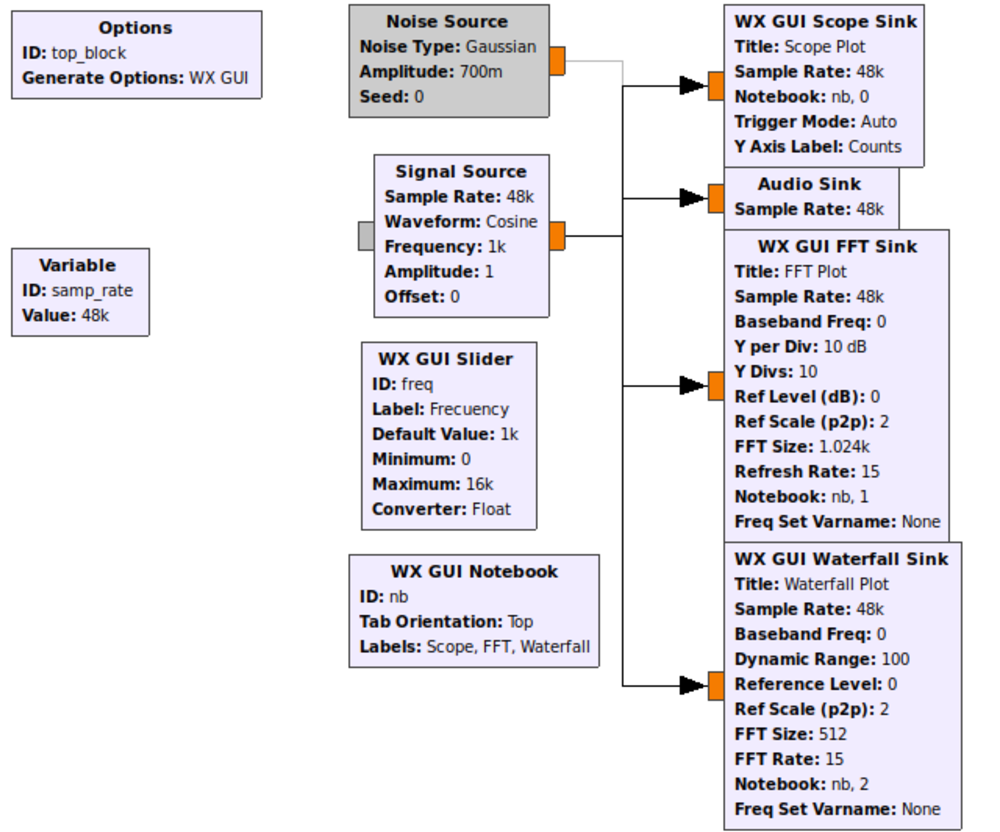
\includegraphics[width=.7\textwidth]{parte1/lab4/pdf/lab4_1.pdf}
\end{center}
\end{figure}

\end{frame}
%----------------

\begin{frame}{Diagrama:  ``emisión de audio desde la computadora''\index{Audio}}

\begin{figure}

\begin{center}
\vspace{-2mm}
    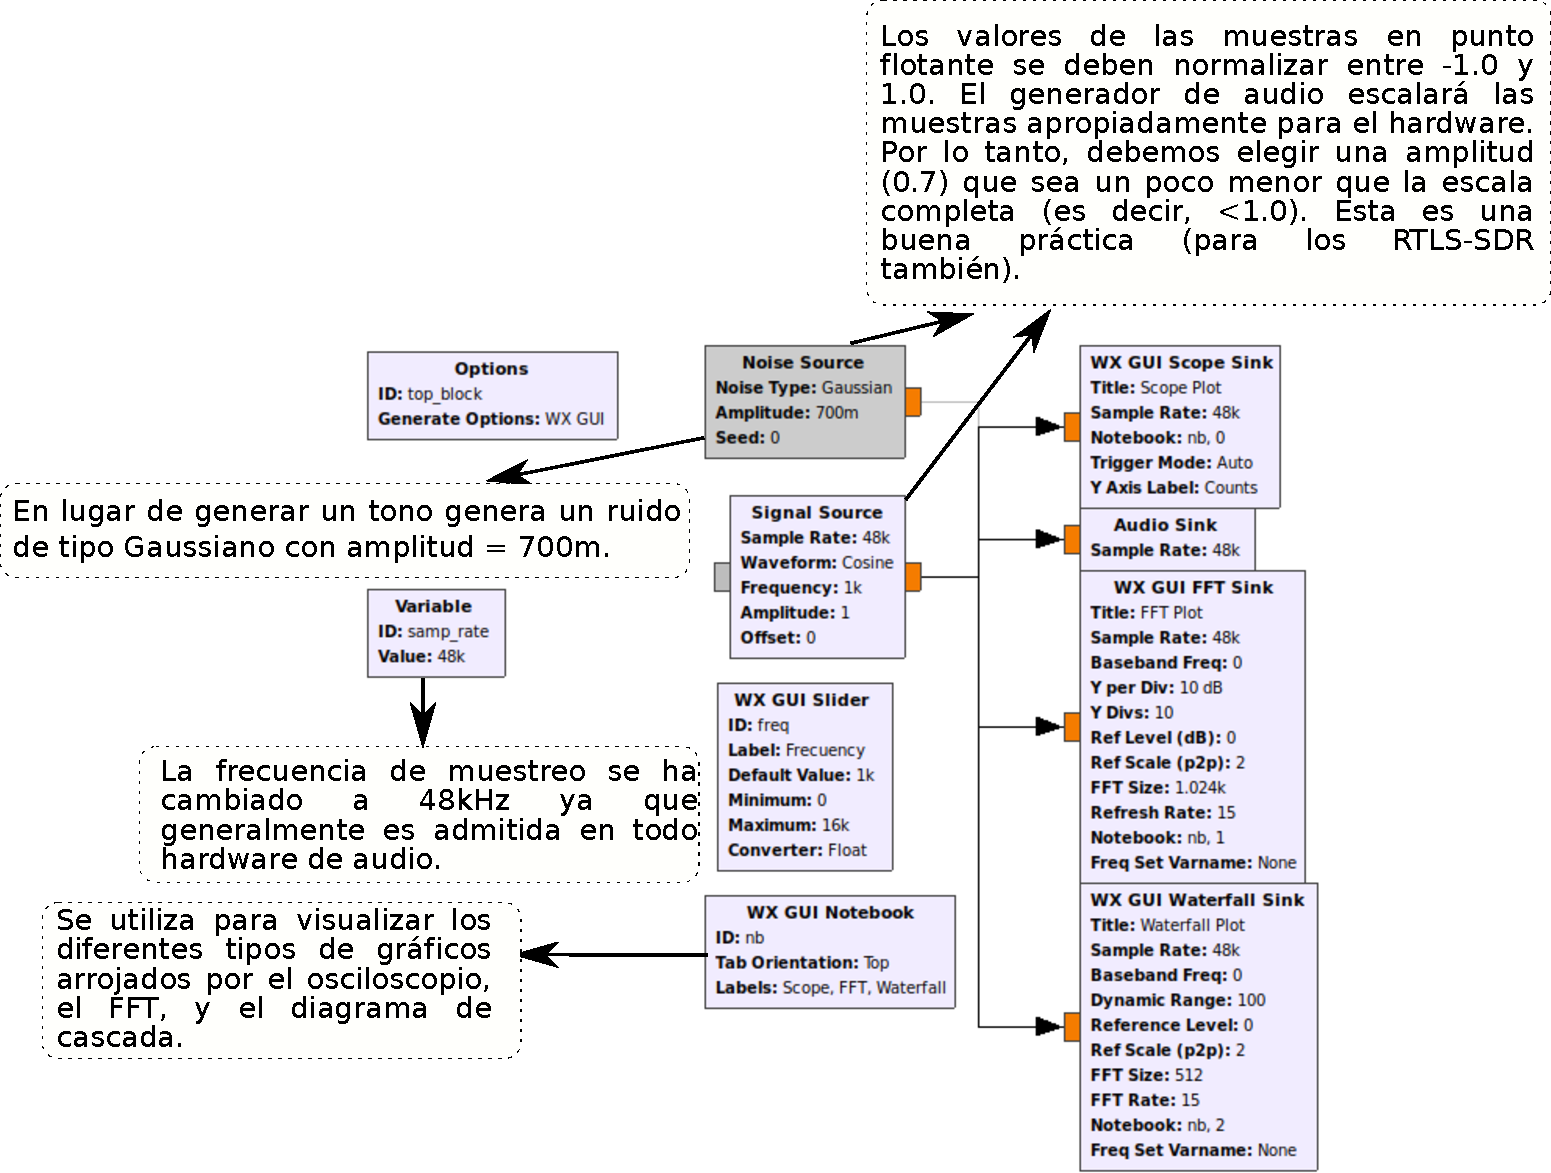
\includegraphics[width=.85\textwidth]{parte1/lab4/pdf/lab4_2.pdf}
\end{center}
\end{figure}

\end{frame}
%----------------

\begin{frame}{Diagrama:  ``emisión de audio desde la computadora''\index{Audio}}

\begin{figure}

\begin{center}
\vspace{-1mm}
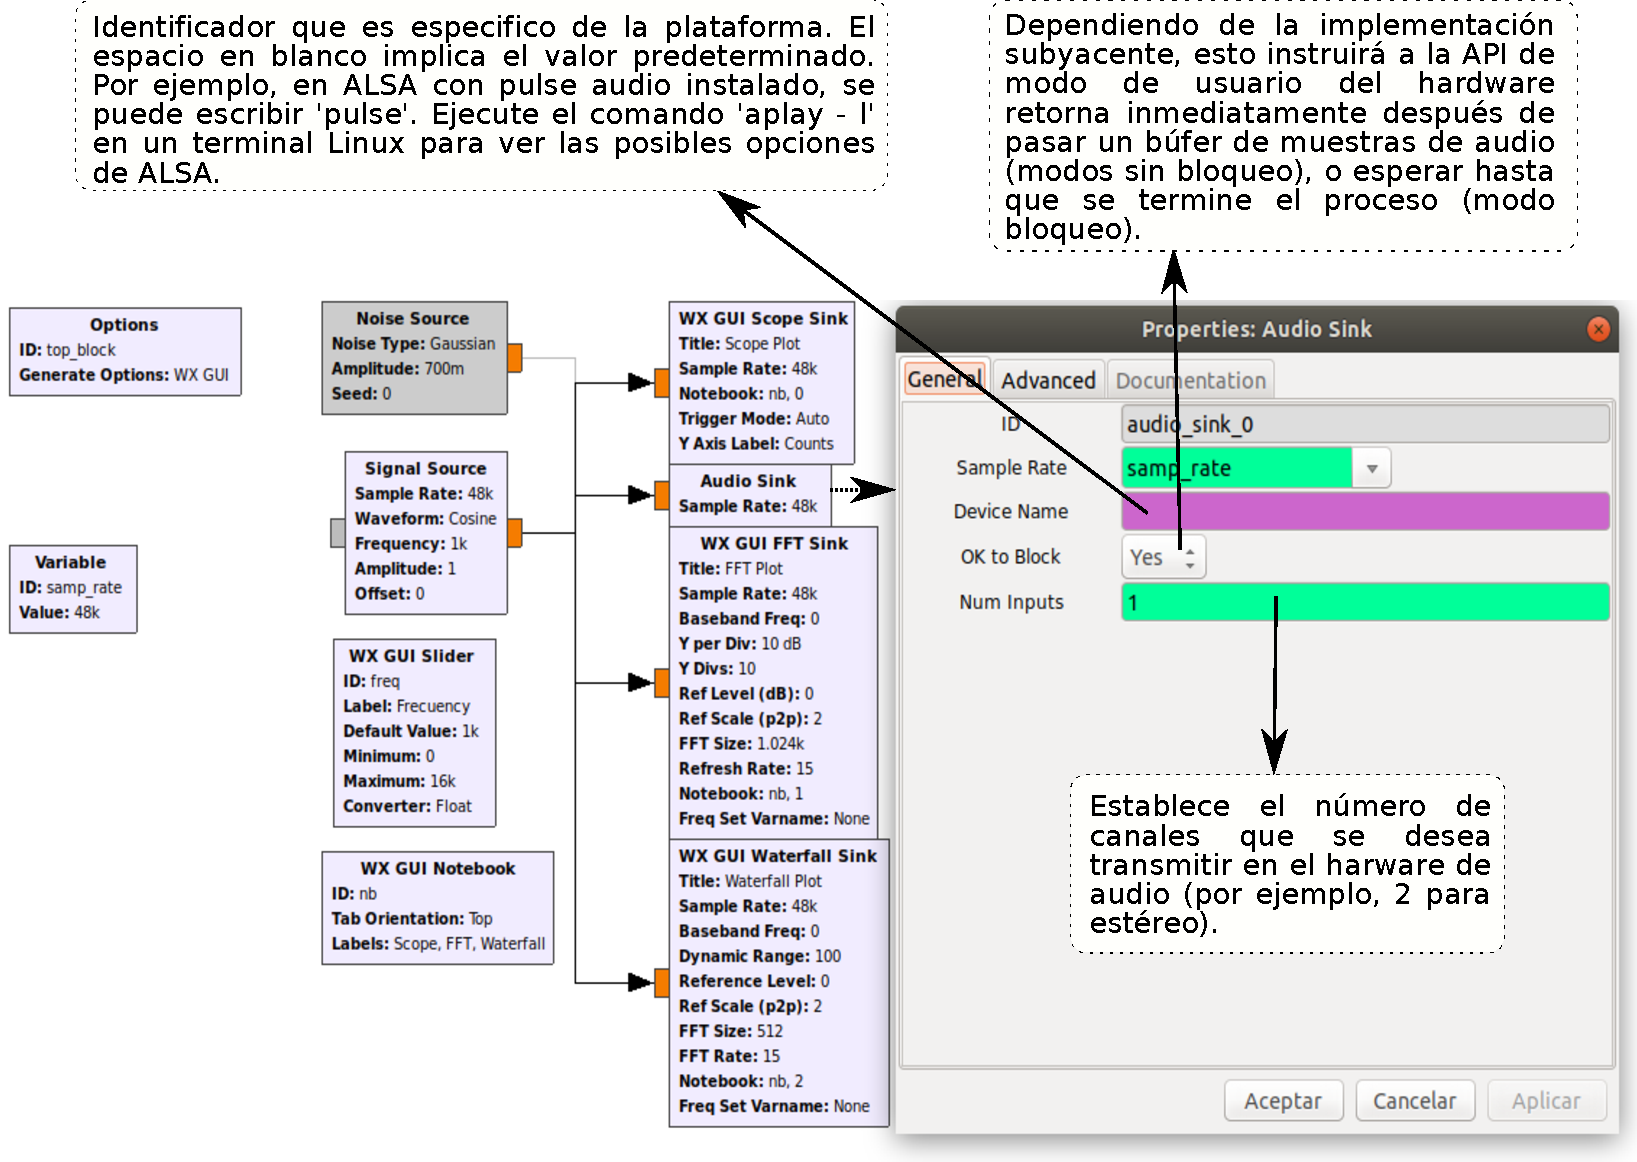
\includegraphics[width=.92\textwidth]{parte1/lab4/pdf/lab4_3.pdf}
\end{center}
\end{figure}

\end{frame}
%----------------

\begin{frame}{Diagrama:  ``emisión de audio desde la computadora''\index{Audio}}

\begin{figure}

\begin{center}
\vspace{-8mm}
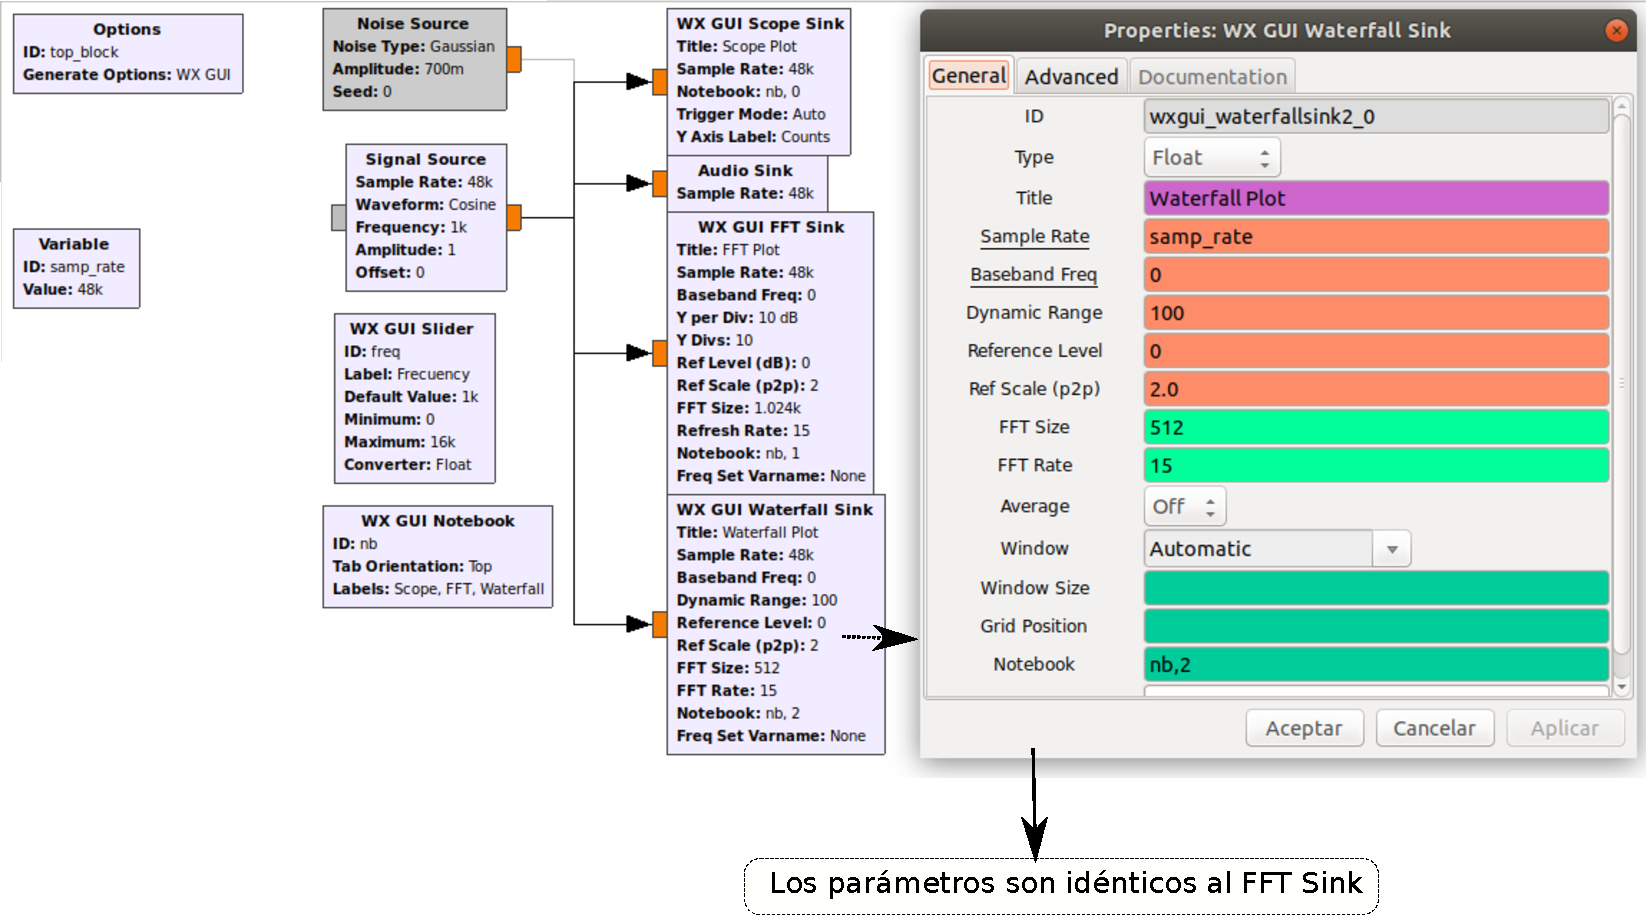
\includegraphics[width=1.05\textwidth]{parte1/lab4/pdf/lab4_4.pdf}
\end{center}
\end{figure}

\end{frame}
%----------------

\begin{frame}{Audio\index{Audio}}

Es importante saber que:\\
\begin{itemize}
    \item
    {Cuando Audio Sink es el único dispositivo hardware en el diagrama de bloques capaz de generar audio, el modo de bloqueo (‘OK to Block’) aplicará un regulador a la producción de muestras del sample\_rate, para que opere eficazmente al reproducir el sonido\cite{Seeber2014}.}
    \item
    {Esto puede ser problemático si la fuente del diagrama de flujo es, por ejemplo, un RTL-SDR. La fuente es también un hardware que tiene su propio reloj interno y será regulado a la tasa de producción de las muestras, mientras que el Audio Sink regula el uso con su propio reloj no sincronizado. Esto se llama el problema de “dos relojes".}
\end{itemize}
\end{frame}
%----------------

\begin{frame}{Audio\index{Audio}}
\begin{itemize}
    \item 
    {Para solucionar este problema de dos relojes, se coloca un regulador de audio en modo sin bloqueo (no dar click ‘Botón de Bloqueo’) de tal forma que nunca interrumpa el diagrama de bloque (es decir, no aplicar el regulador controlado). Esto usará muestras de forma normal, pero si hay un exceso (por ejemplo, el RTL-SDR está produciendo muestras un poco más rápido de lo que el Audio Sink puede usar), se perderán las muestras (podría causar fallas de audio).}
    \item 
    {Esto no soluciona el caso en el que las muestras se producen más lentamente que la tasa de uso del Audio Sink (esto producirá una ejecución lenta: el audio sonará agitado y se imprimirá ‘aU’ en la ventana de registro).}
\end{itemize}



\end{frame}
%----------------

\begin{frame}{Audio\index{Audio}}

\begin{figure}

\begin{center}
\vspace{-7mm}
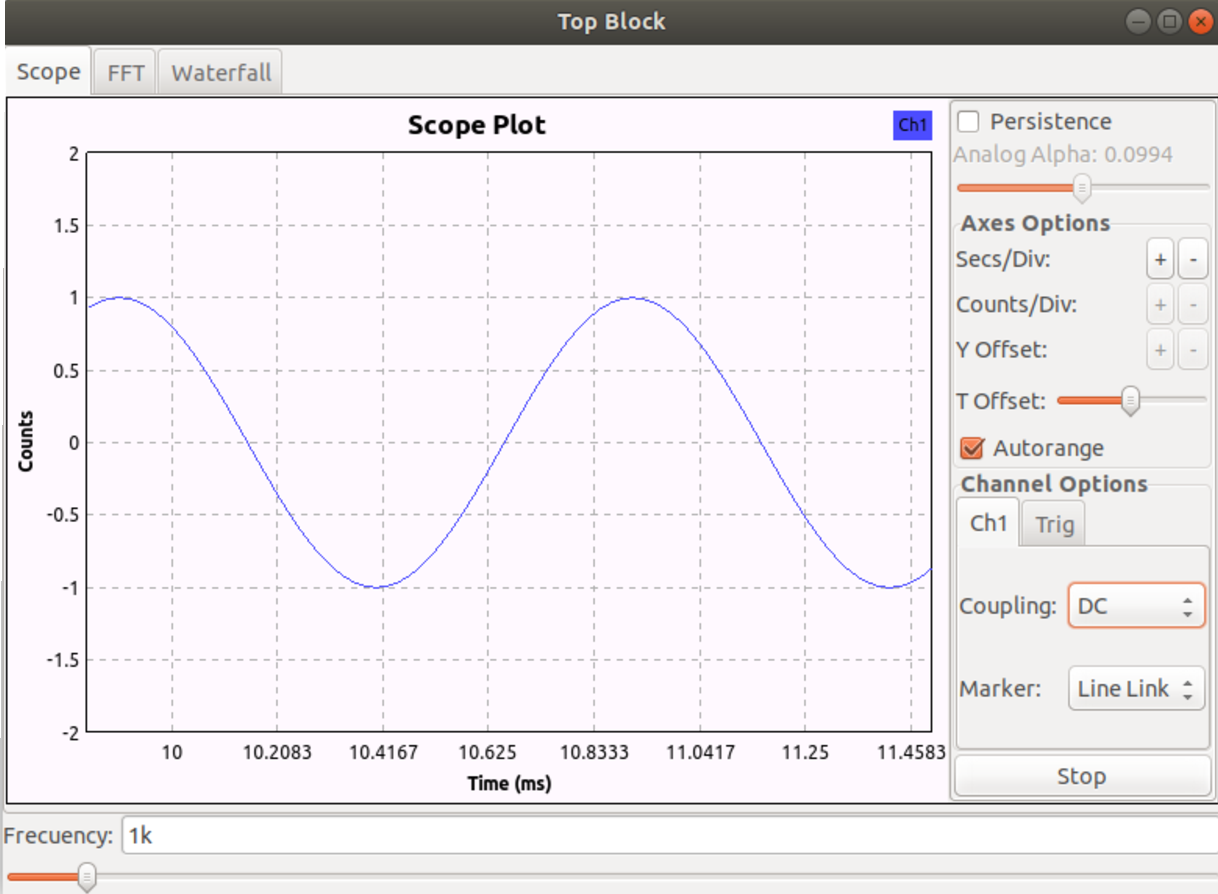
\includegraphics[width=\textwidth, height=0.6\paperheight]{parte1/lab4/pdf/lab4_5.pdf}
\end{center}
\end{figure}
%\tiny
\vspace{-4mm}
La misma onda seno de las prácticas anteriores, pero ahora se puede escuchar emitida por los parlantes del computador.
\end{frame}
%----------------

\begin{frame}{Audio\index{Audio}}

\begin{figure}

\begin{center}
\vspace{-6mm}
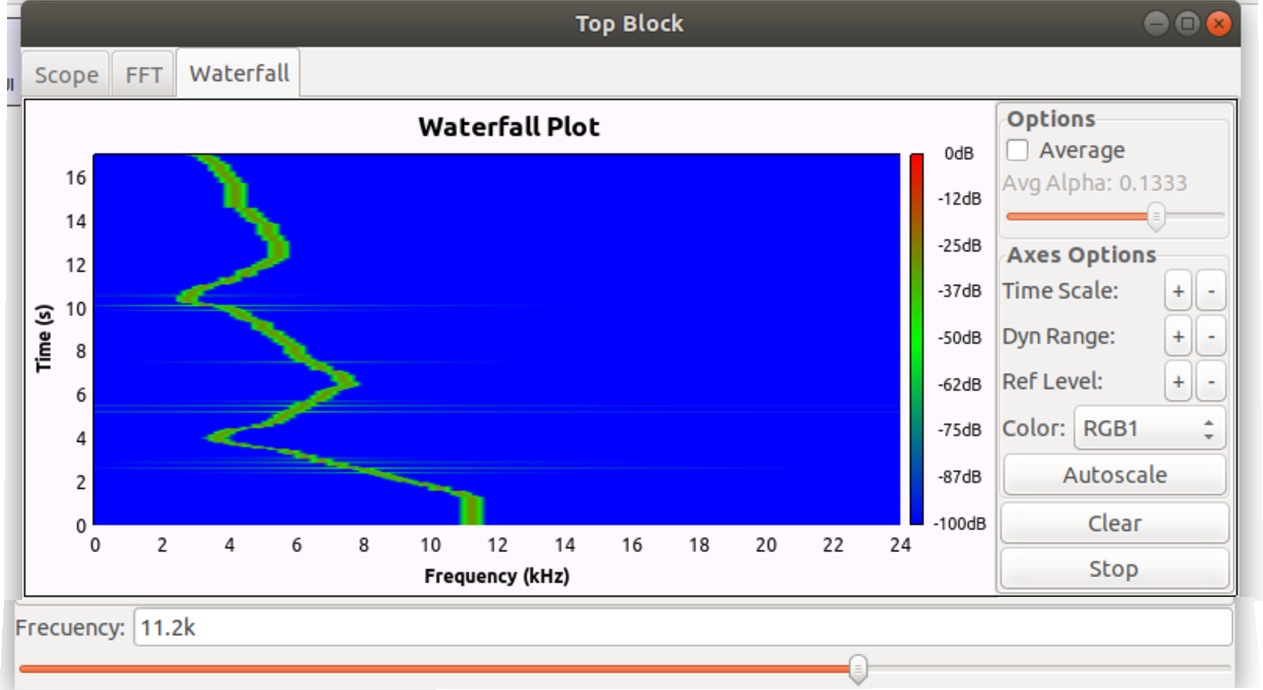
\includegraphics[width=0.8\textwidth]{parte1/lab4/pdf/lab4_6.pdf}
\end{center}
\end{figure}
\vspace{-3mm}

Visualiza el FFT que se desplaza en el tiempo mediante el diagrama de cascada (espectrograma) de la señal emitida. Se añade un bloque de prueba por medio de un generador de señales y un variador deslizante con lo cual se escucha el tono variado en el Audio Sink y poder ver la variación de la frecuencia en el diagrama de cascada.
\end{frame}
%----------------

\begin{frame}{Diagrama: recepción de audio\index{Audio}}

\begin{figure}

\begin{center}
%\vspace{-5mm}
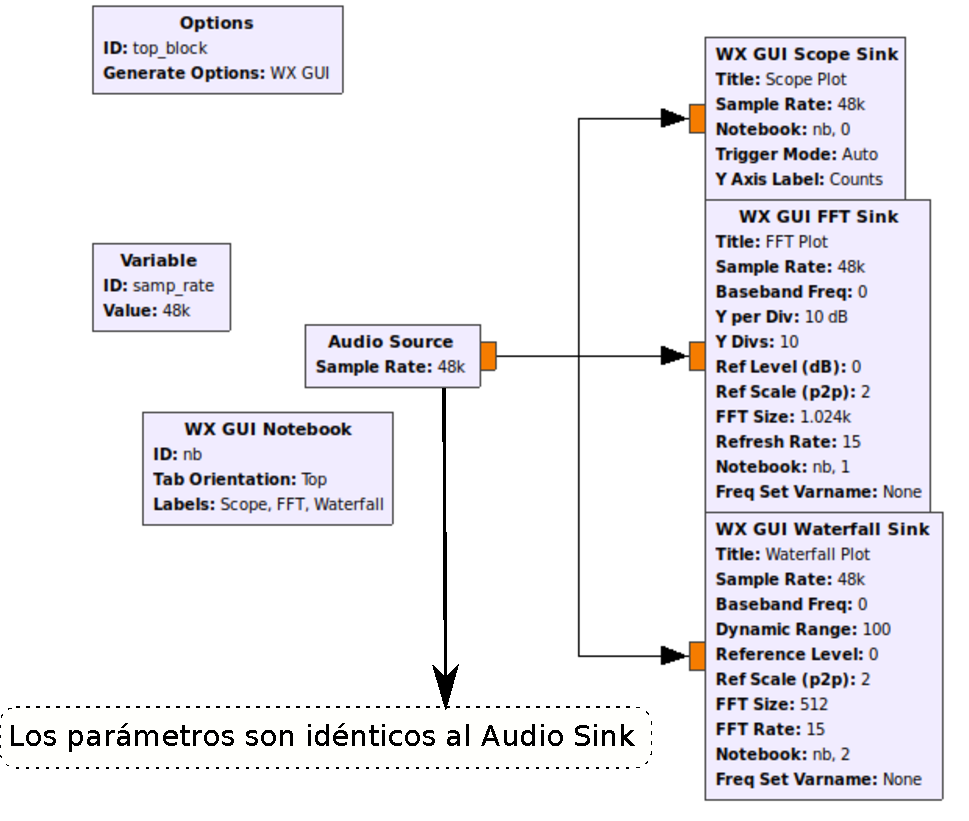
\includegraphics[width=.73\textwidth]{parte1/lab4/pdf/lab4_7.pdf}
\end{center}
\end{figure}

\end{frame}
%----------------

\begin{frame}{Audio\index{Audio}}

\begin{figure}
\begin{center}
\vspace{-8mm}
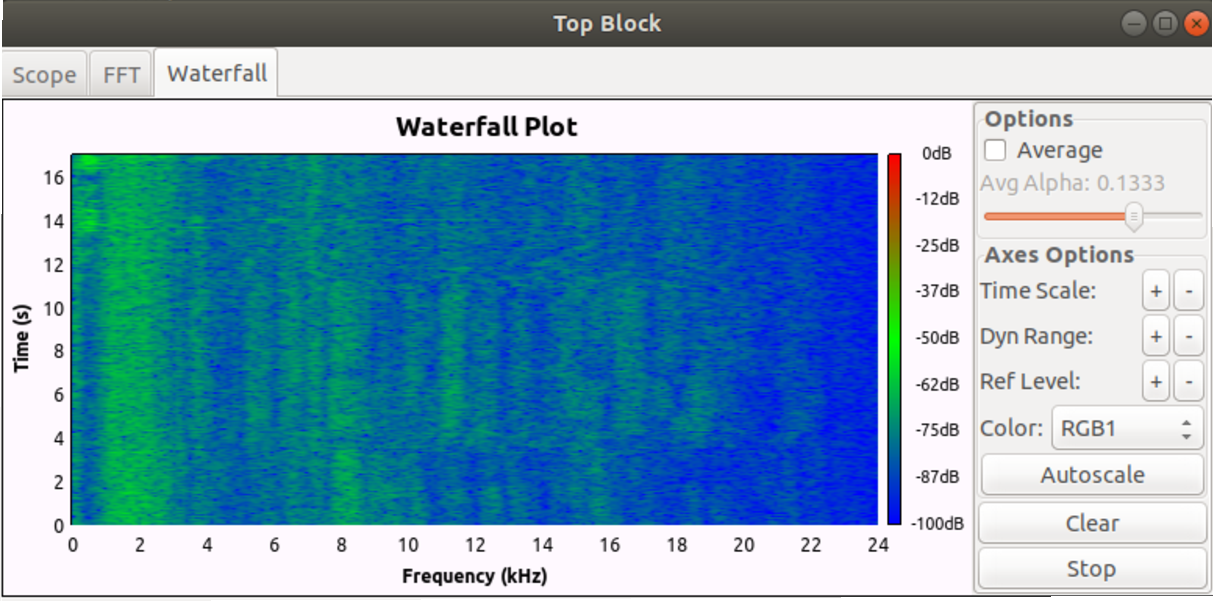
\includegraphics[width=\textwidth]{parte1/lab4/pdf/lab4_8.pdf}
\end{center}
\end{figure}

Muestra las diferentes señales presentes en el entorno captadas por la tarjeta de audio de la computadora a través del micrófono.

\end{frame}
%----------------

\begin{frame}{Diagrama: prueba con aproximación de “loopback”\index{Audio}}

\begin{figure}
\begin{center}
\vspace{-6mm}
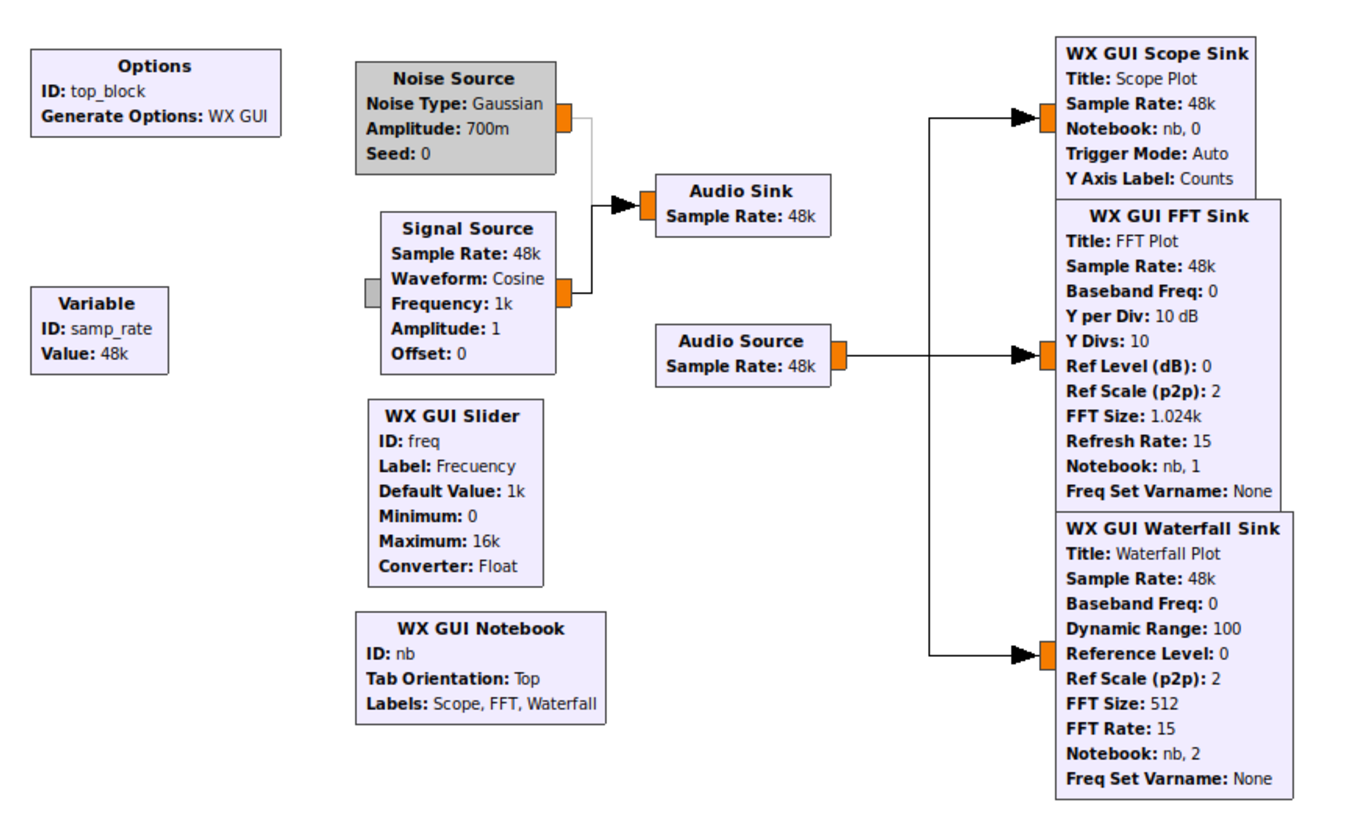
\includegraphics[width=\textwidth, height=0.6\paperheight]{parte1/lab4/pdf/lab4_9.pdf}
\end{center}
\end{figure}
\vspace{-5mm}
Ejecutando el programa generador de onda sinusoidal al mismo tiempo, y cambiando la frecuencia. Se trata de una prueba aproximada de “loopback" en la que el micrófono de la computadora escucha sus altavoces.

\end{frame}
%----------------

\begin{frame}{Audio\index{Audio}}

\begin{figure}
\begin{center}
\vspace{-8mm}
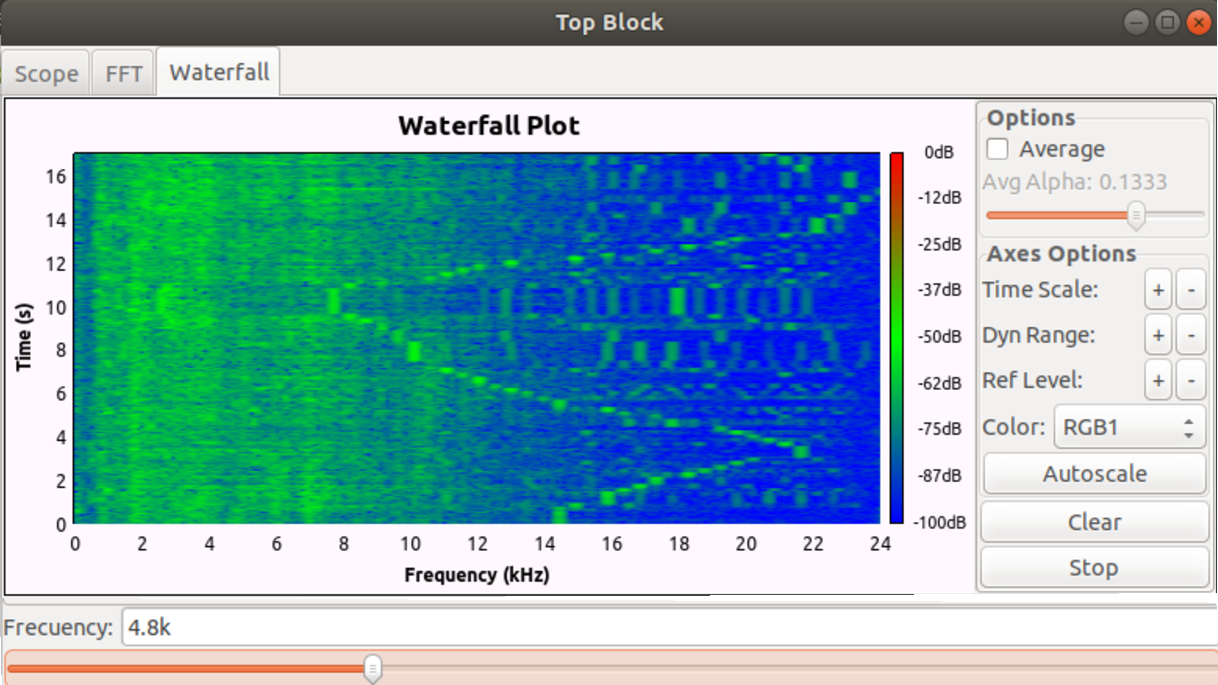
\includegraphics[width=\textwidth, height=0.6\paperheight]{parte1/lab4/pdf/lab4_10.pdf}
\end{center}
\end{figure}
\vspace{-5mm}
Con la realimentación de las entradas micrófono-altavoces y generación de señal a través de la tarjeta de audio de la computadora.

\end{frame}
%---------------

\begin{frame}{ERRORES DE SINCRONIZACION}

Los datos de frecuencias de muestreo a un receptor de audio funcionan a 48000S/s muestras por segundo, aunque no todos los receptores pueden ser manejados en esta frecuencia. Dependiendo de la unidad de audio utilizada y el hardware, algún día se produce un overflow o underflow del búfer, imprimiendo uno de los siguientes códigos de error:\\ \vspace{2mm}


\begin{description}
   
\item["a"] audio (tarjeta de sonido).\\ \vspace{2mm}
\item["O"]overrrun “desbordamiento” (la PC no se mantiene al día con los datos recibidos de la tarjeta de audio usrpor). \\ \vspace{2mm}
\item["U"] underrun “subestimada” (la PC no proporciona datos lo suficientemente rápido).\\ \vspace{2mm}


\end{description}

\end{frame}
%---------------

\begin{frame}{ERRORES DE SINCRONIZACION}

\begin{description}


\item["aUaU"]audio underrun (no hay suficientes muestras listas para enviar al sonido USRPsink).\\ \vspace{2mm}
\item["uOuO"]USRP desbordado (las muestras de USRP se descartaron porque no se leyeron a tiempo). \\ \vspace{2mm}
\item["S"] indica un error de número de secuencia en los paquetes de Ethernet que marca una saturación de USRP a la PC como “O”.\\ \vspace{2mm}


\end{description}

La arquitectura de audio más común utilizada en Linux es ”Arquitectura de sonido avanzada de Linux” (ALSA). Incluye un dispositivo de muestreador de software llamado plughw, que proporciona una amplia adaptación de frecuencia en un rango dado.\\ \vspace{2mm}

\end{frame}
%---------------
\begin{frame}{ERRORES DE SINCRONIZACION}

\begin{figure}
\begin{center}
\vspace{-8mm}
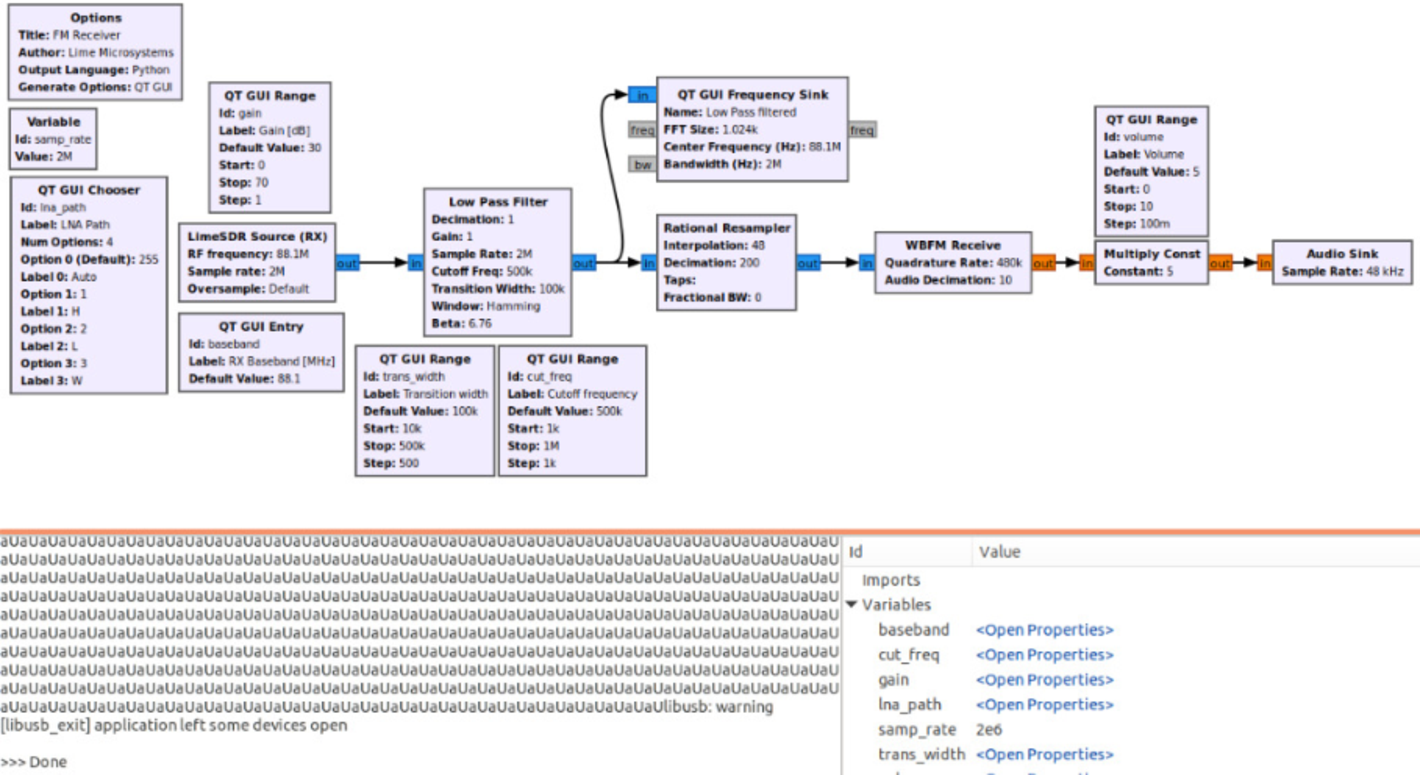
\includegraphics[width=\textwidth, height=0.6\paperheight]{parte1/lab4/pdf/aUaU.pdf}
\end{center}
\end{figure}
\vspace{-5mm}


\end{frame}
%---------------
\begin{frame}{ERRORES DE SINCRONIZACION}

cuando nos aparece este error “aUaU” lo más probable es que sea un ”problema de 2 relojes”. El problema es que tiene 2 piezas de hardware con un reloj, y no hay forma de alinearlas o sincronizarlas perfectamente. Aquí hay muchos modos de falla, pero uno muy obvio es el siguiente: imagine que el radio reloj (emisor) es un poco más lento de lo anunciado, y el reloj de audio (receptor) es más rápido.por lo tanto en algun momento la cantidad de datos subministrados seran muy bajos tanto asi que se perderan dichos datos y nos aparecera dicho error. Además, recuerde que GNU Radio mezcla datos en fragmentos, por lo que puede haber
suficientes datos, pero no en el momento preciso en que el receptor de audio los necesita.\\ \vspace{2mm}

\end{frame}
%---------------
\begin{frame}{ERRORES DE SINCRONIZACION}

una posible solucion es verificar que todos los bloque esten funcionando de forma predeterminada y que no hallan sufrido cambios debido a que esto podria generar una variacion de velocidad en los relojes.\\ \vspace{2mm}

Este error solo ocurrira cuando estemos trabajando dos dispositivos con su respectivo reloj (tarjeta de audio, RTL, etc) o siempre y cuando tengamos un emisor y un receptor y la velocidad de su reloj o procesamiento sea muy diferente.\\ \vspace{2mm}

\end{frame}
%---------------

\begin{frame}{ERRORES DE SINCRONIZACION}

El muestreo a una frecuencia de muestreo alta puede causar errores de desbordamiento, lo que significa que la computadora host no puede procesar las muestras entrantes a la frecuencia que se entregan, lo que nuevamente significa que el USRP tiene que descartar las muestras. Por lo general, esto lo detecta el software de manejo y se le notifica al usuario imprimiendo ”O” sutil en la salida estándar. \\ \vspace{2mm}

Sin embargo, el autor no los buscó, especialmente porque no se esperaba un desbordamiento para las frecuencias de muestreo a 1 MHz. Debido a la incertidumbre, el autor tuvo que retroceder y medir ambas balizas a diferentes frecuencias de muestreo para evitar por completo la posibilidad de que LA2SHF tuviera problemas de tiempo en su código Morse, y que esto era solo desbordamientos y errores de tiempo durante nuestra recepción cadena.\\ \vspace{2mm}

\end{frame}


%---------------
\begin{frame}{ERRORES DE SINCRONIZACION}

\begin{figure}
\begin{center}
\vspace{-8mm}
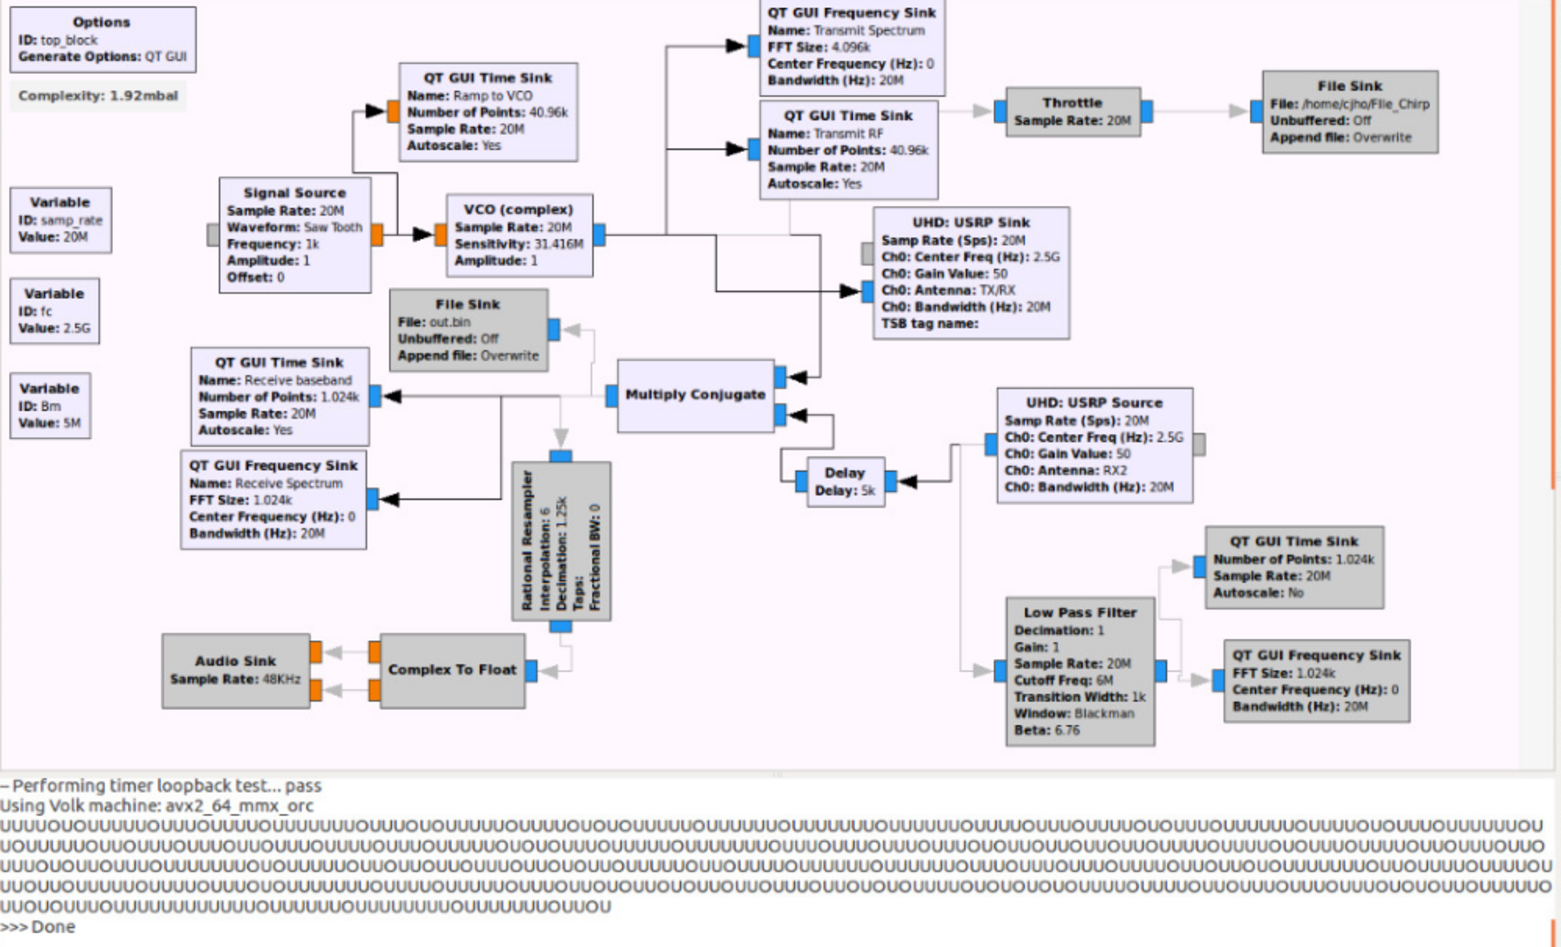
\includegraphics[width=\textwidth, height=0.6\paperheight]{parte1/lab4/pdf/OUOU.pdf}
\end{center}
\end{figure}
\vspace{-5mm}

uOuO = USRP desbordado (las muestras de USRP se descartaron porque no se leyeron a tiempo.\\ \vspace{2mm}

\end{frame}
%---------------
\begin{frame}{ERRORES DE SINCRONIZACION}

\begin{figure}
\begin{center}
\vspace{-8mm}
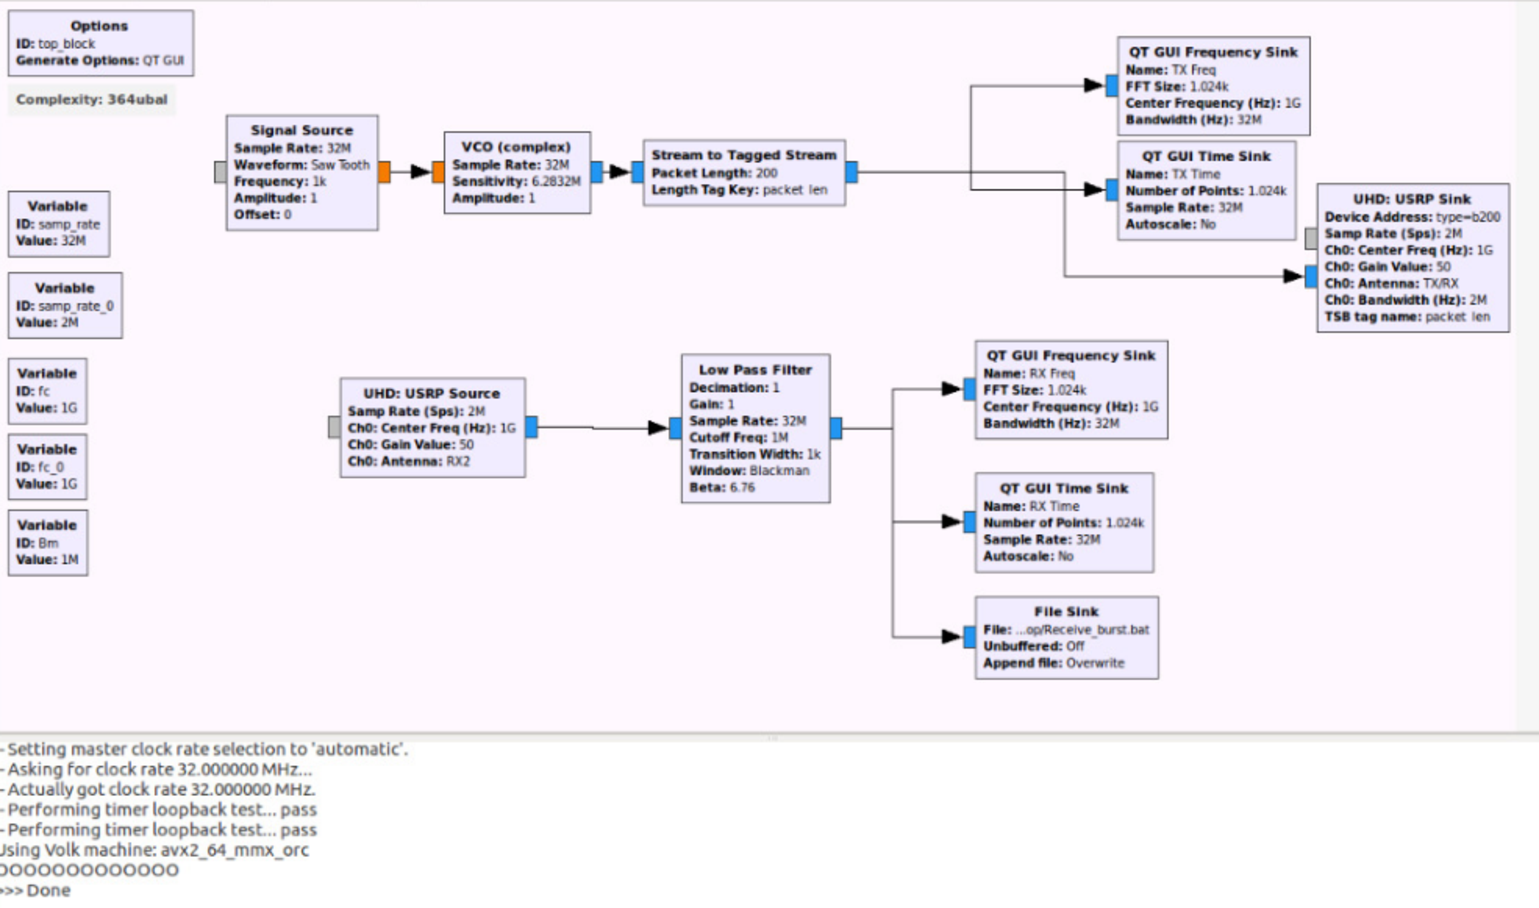
\includegraphics[width=\textwidth, height=0.6\paperheight]{parte1/lab4/pdf/OOO.pdf}
\end{center}
\end{figure}
\vspace{-5mm}


\end{frame}
%---------------

\begin{frame}{ERRORES DE SINCRONIZACION}

El hecho de que el problema de sincronización se debe a desbordamientos también es muy evidente por el hecho de que el diagrama de flujo de GNU Radio imprimió ”OOO” durante la recepción de esta serie de mediciones, lo que indica al menos tres desbordamientos, lo que notamos si hubiéramos seguido la salida
estándar de GNU Radio acompañante más diligentemente durante las mediciones del patrón. \\ \vspace{2mm}

Esto no es muy interesante, y es un problema conocido que debe tenerse en cuenta asegurando que la computadora esté al día, que los bloques puedan manejar la transmisión, que la conexión al USRP sea lo suficientemente rápida, etc.\\ \vspace{2mm}

\end{frame}


%---------------


